% -----------------------------------------------------------------------------
% COPYRIGHT & INTELLECTUAL PROPERTY NOTICE
% -----------------------------------------------------------------------------
% File: paper.tex
% Author: [Chia-Tuan Chang] (Independent Researcher)
% Date: 2026
%
% © 2026 [Chia-Tuan Chang]. ALL RIGHTS RESERVED.
%
% This document source (.tex) is the proprietary intellectual property of 
% the author. It is currently under peer-review for academic publication 
% (SIGBOVIK).
%
% RESTRICTIONS:
% 1. NO REDISTRIBUTION: This source file may not be redistributed, mirrored, 
%    or hosted on any other platform without express written permission.
% 2. NO MODIFICATION: Any unauthorized modification, remixing, or building 
%    upon this source code is strictly prohibited.
% 3. CITATION: Any reference to the theorems, proofs, or algebraic structures 
%    defined herein must cite the official publication or the corresponding 
%    arXiv preprint (once available).
%
% CONTACT: For licensing inquiries, please contact the author via this 
% GitHub repository or associated official channels.
% -----------------------------------------------------------------------------

% The Pareto-Minkowski Semiring of Hatsune Miku
% For submission to SIGBOVIK 2026

\documentclass[11pt, letterpaper]{article}

\usepackage{xcolor}
\definecolor{MikuCyan}{RGB}{57, 197, 187}

\usepackage[margin=1in]{geometry}
\usepackage{amsmath, amssymb, amsthm}
\usepackage{url}
\usepackage{booktabs}
\usepackage{enumitem}
\usepackage{graphicx}
\usepackage{tikz}
\usepackage{CJKutf8}
\usepackage[
    colorlinks=true, % 開啟文字上色，關閉預設超醜的彩色方框
    linkcolor=MikuCyan, % 內部連結
    citecolor=MikuCyan, % 參考文獻連結
    urlcolor=MikuCyan, % 外部網址連結
    filecolor=MikuCyan, % 本地檔案連結
    pdfborder={0 0 0} % 確保在某些舊版閱讀器中也不會出現邊框
]{hyperref}

% 字體(Linux Libertine)
\usepackage[T1]{fontenc} % 確保字體編碼正確，處理連字
\usepackage{libertine} % 將主要文字換成Linux Libertine，無襯線字體換成Biolinum
\usepackage[libertine]{newtxmath} % 讓數學公式的字體與Libertine搭配

\newtheorem{theorem}{Theorem}
\newtheorem{lemma}[theorem]{Lemma}
\newtheorem{proposition}[theorem]{Proposition}
\newtheorem{corollary}[theorem]{Corollary}
\theoremstyle{definition}
\newtheorem{definition}[theorem]{Definition}
\theoremstyle{remark}
\newtheorem{remark}[theorem]{Remark}

% ================================================================
\title{The Pareto-Minkowski Semiring of Hatsune Miku:\\
How She Accidentally Invented $\mathrm{FL^{NL}}$}
\author{Chia-Tuan Chang\\
\small Independent Researcher, Taipei, Taiwan (ROC)\\
\small \texttt{changchiatuan@gmail.com}}
\date{}

% ================================================================
\begin{document}
\maketitle
\pagestyle{empty}
\thispagestyle{empty}

% ================================================================
\begin{abstract}
We revisit the score maximization problem in an arcade rhythm game: \textit{Hatsune Miku: Project DIVA Arcade} (PDA), previously argued in a companion manuscript to be polynomial-time solvable and to lie in NC$^2$ via parallel transfer-function composition.
We observe that the underlying computation possesses a natural algebraic structure: the set of Pareto frontiers over non-negative integer pairs forms a semiring, specifically an additively idempotent semiring (dioid), under union-then-Pareto-prune as addition and Minkowski-sum-then-Pareto-prune as multiplication.
We call this the \emph{Pareto-Minkowski semiring} (or, in honour of its application domain, the \emph{Hatsune semiring}).
Under this lens, the transfer-function composition becomes iterated matrix multiplication over a semiring, directly connecting rhythm game optimization to the classical theory of algebraic path problems.
We further refine the complexity classification by showing that the decision version lies in NL and the search version in $\mathrm{FL^{NL}}$, obtaining the tighter upper bound of NL within NC$^2$.
These results demonstrate that SEGA's scoring system, while appearing fiendishly complex to players, inhabits a remarkably well-studied algebraic and complexity-theoretic landscape.
\end{abstract}

\smallskip
\noindent\textbf{Keywords:} semiring theory, dioid, Pareto optimality, Minkowski sum, algebraic path problems, multi-objective optimization, nondeterministic logspace (NL), $\mathrm{FL^{NL}}$, $\mathrm{NC}^2$, rhythm games, Hatsune Miku

% ================================================================
\section{Introduction: The Odd One Out}

Hatsune Miku is, to our knowledge, the first virtual pop star whose scoring system has been rigorously shown to inhabit $\mathrm{FL^{NL}}$.

In the vast majority of arcade rhythm games: \textit{maimai}, \textit{CHUNITHM}, \textit{Sound Voltex}, and their brethren, the path to the highest score is utterly boring from a complexity-theoretic standpoint.
Each note is locally independent: hitting it perfectly is always at least as good as any alternative.
The score maximization problem reduces to ``hit everything perfectly,'' which a constant-depth threshold circuit can verify.
Formally, these problems reside in TC$^0$ \cite{Chang2026}, the computational equivalent of barely having to think.

\textit{Hatsune Miku: Project DIVA Arcade} (PDA) \cite{DivaAcWiki, ProjectDivaWiki} is the black sheep of this family (Figure~\ref{fig:cabinet}).

\begin{figure}[h!]
    \centering
    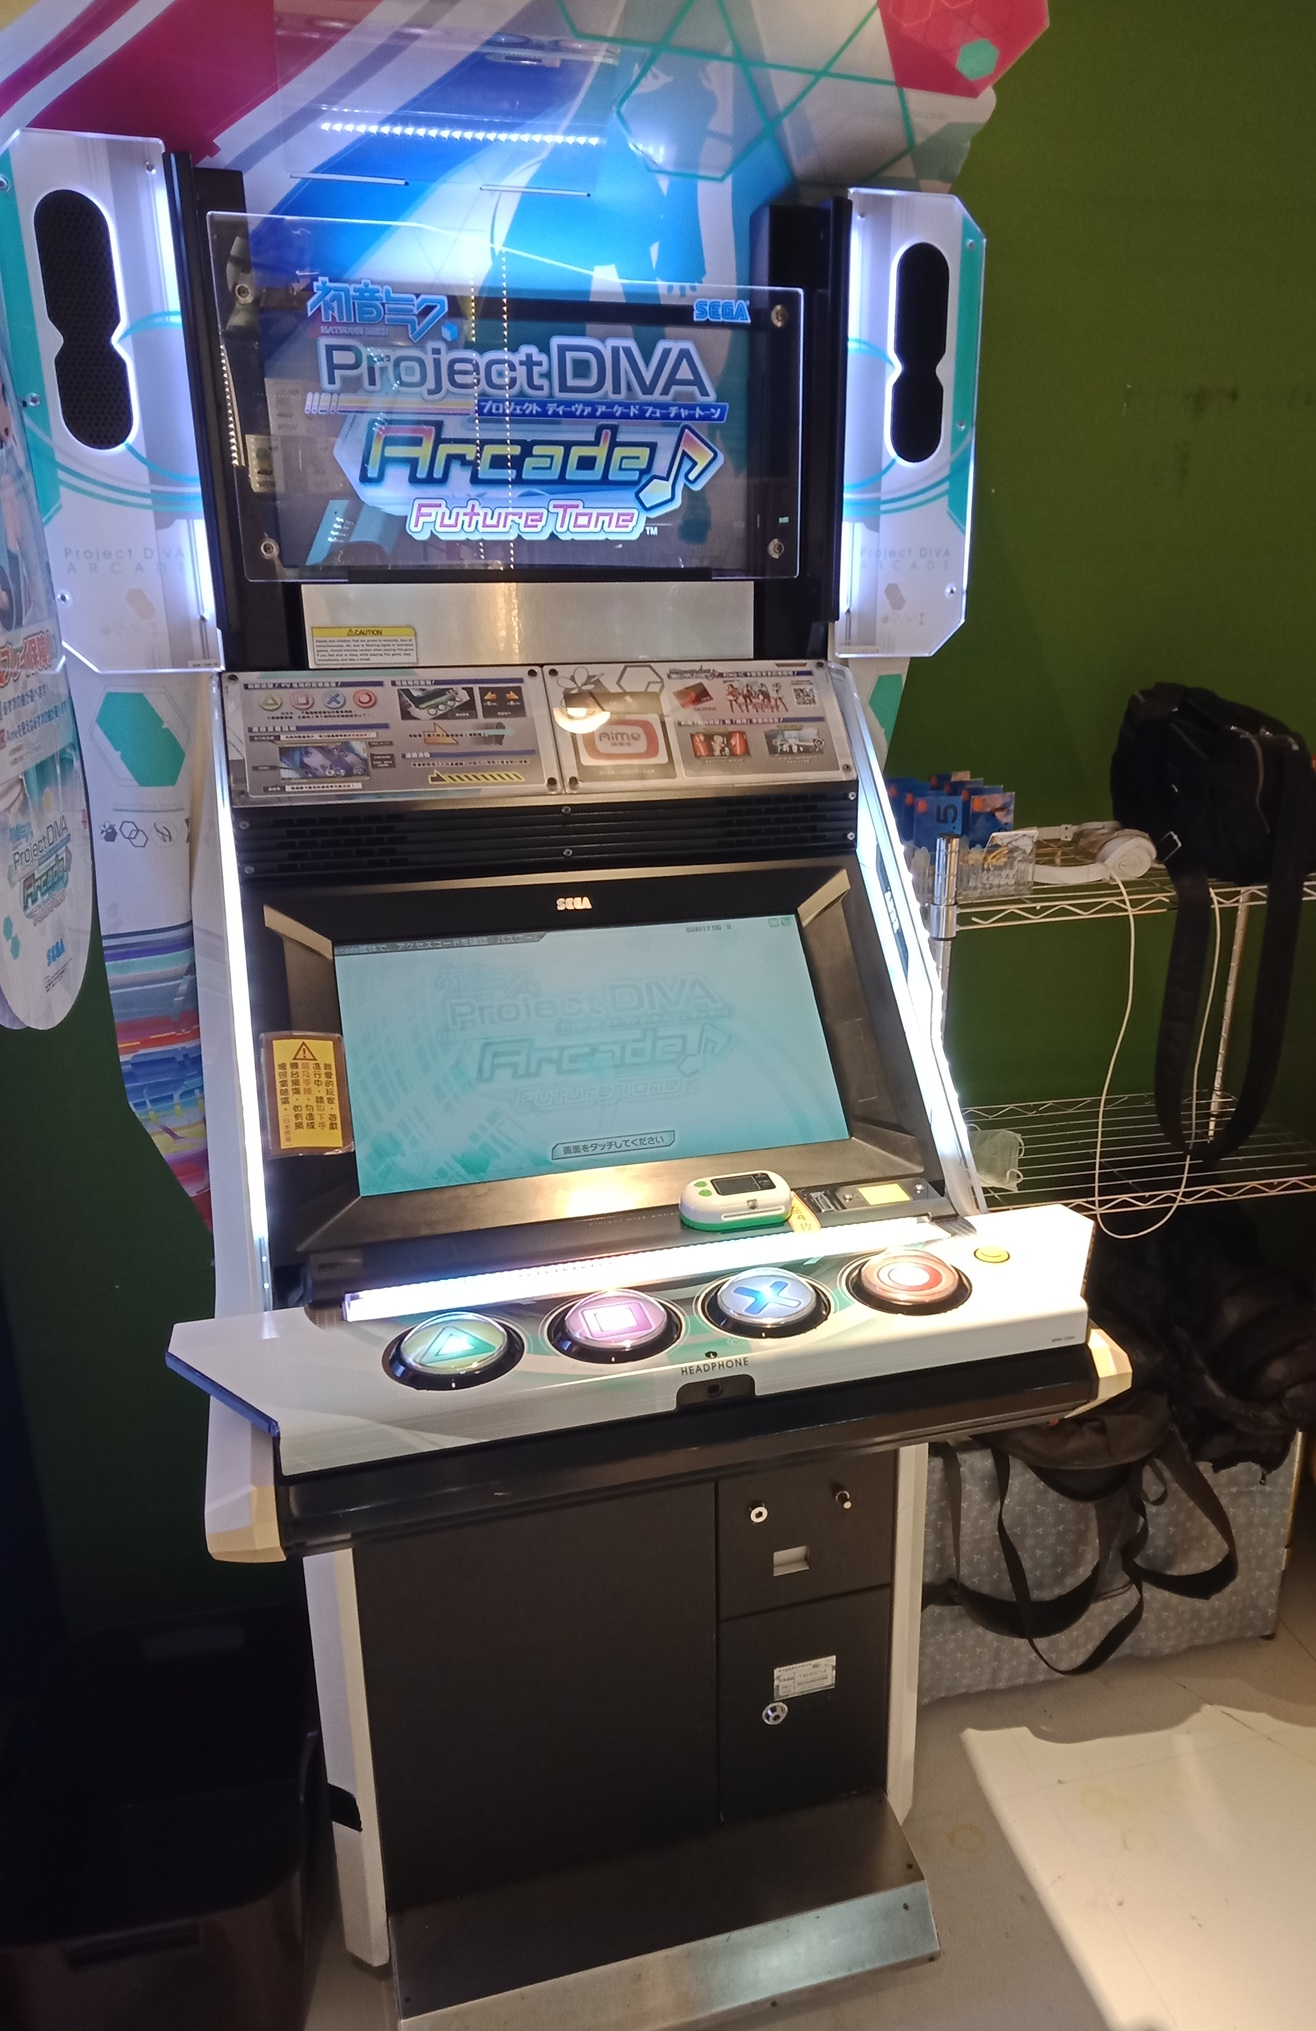
\includegraphics[width=0.5\linewidth]{figures/cabinet.jpg}
    \caption{A \textit{Hatsune Miku: Project DIVA Arcade} cabinet in the wild.
    The four coloured buttons (\textbf{$\bigcirc$}, \textbf{$\times$}, \textbf{$\square$}, \textbf{$\triangle$}) and the slide bar are the entire input alphabet of our optimization problem.}
    \label{fig:cabinet}
\end{figure}
Its \emph{Shared Release Constraint} (Figure~\ref{fig:src}), whereby releasing any button during a multi-button hold terminates \emph{all} active holds simultaneously, creates genuine inter-note dependencies.
Hitting a note perfectly can, paradoxically, cost thousands of points by prematurely terminating a lucrative hold sequence.
To make matters more interesting, PDA imposes a strict life gauge (reach zero and it is Game Over), and requires the player's \emph{achievement rate} (a piecewise-linear function of both the total score and the hold score) to exceed a difficulty-dependent threshold upon song completion.
This is not a single-objective optimization problem with a greedy solution, it is a constrained bi-objective optimization problem demanding global reasoning across the entire chart.

In a recent manuscript currently under review \cite{Chang2026}, we formalized this as the Project DIVA Optimization Problem (PDOP) and proved that it is solvable in polynomial time via dynamic programming ($O(m^2 \log m)$ for a chart with $m$ notes).
We further showed PDOP $\in$ NC$^2$ by demonstrating that the DP admits parallelization via balanced binary-tree composition of transfer functions, achieving $O(\log^2 m)$ parallel depth.
That work focused on algorithms and complexity classifications, centring on the \emph{how fast can we solve it?}\ question.

The present paper takes a different tack.
Rather than algorithms, we are interested in \emph{algebra}: the \emph{what is the mathematical structure?}\ question.
We strip away the game-specific details and expose the elegant structure lurking beneath:
\begin{enumerate}[leftmargin=*]
    \item We identify the \textbf{Pareto-Minkowski semiring} $(\mathcal{P},\, \oplus,\, \otimes,\, \mathbf{0},\, \mathbf{1})$, an additively idempotent semiring (dioid) whose elements are anti-chains of $\mathbb{N}_0^2$, with Pareto-pruned union as addition and Pareto-pruned Minkowski sum as multiplication (Section~\ref{sec:semiring}).
    \item We show that the transfer-function composition from \cite{Chang2026} is \emph{exactly} matrix multiplication over this semiring, connecting PDA to the classical framework of \emph{algebraic path problems} \cite{Gondran2008, Mohri2002} (Section~\ref{sec:semiring}).
    \item We refine the space complexity of PDOP: the decision version is in \textbf{NL}, and the search version (outputting the optimal decision sequence) is in $\mathbf{FL^{NL}}$. Since NL $\subseteq$ NC$^2$ \cite{Cook1985}, this gives a tighter upper bound than the prior NC$^2$ result (Section~\ref{sec:space}).
\end{enumerate}

To be clear: this paper and \cite{Chang2026} complement each other without overlap.
Reference~\cite{Chang2026} formalizes the game mechanics and proves time/circuit complexity bounds.
This paper identifies the algebraic backbone and establishes space complexity bounds.
If \cite{Chang2026} asks ``how fast?,'' we ask ``what kind of algebra is this, and how little memory does it need?''

For precision, we delineate the provenance of each result:
\begin{center}
\small
\begin{tabular}{@{}lcc@{}}
\toprule
\textbf{Result} & \textbf{\cite{Chang2026}} & \textbf{This paper} \\
\midrule
Game mechanics formalization (Abstract PDA Machine) & $\checkmark$ & --- \\
Bounded state space ($|S| = O(1)$) & $\checkmark$ & cited \\
$O(m^2 \log m)$ DP algorithm (PDOP $\in$ P) & $\checkmark$ & --- \\
PDOP $\in$ NC$^2$ via transfer-function composition & $\checkmark$ & re-derived${}^*$ \\
Pareto-Minkowski semiring: definition \& axioms & --- & $\checkmark$ \\
Matrix formulation over the semiring & --- & $\checkmark$ \\
Connection to algebraic path problems & --- & $\checkmark$ \\
PDOP Decision $\in$ NL & --- & $\checkmark$ \\
PDOP Search $\in$ $\mathrm{FL^{NL}}$ & --- & $\checkmark$ \\
\bottomrule
\end{tabular}
\end{center}
\noindent{\footnotesize ${}^*$The NC$^2$ upper bound is proved independently in \cite[\S4.5]{Chang2026}; here it emerges as a corollary of the semiring-matrix formulation (Section~\ref{sec:semiring}).}

\begin{figure}[h!]
    \centering
    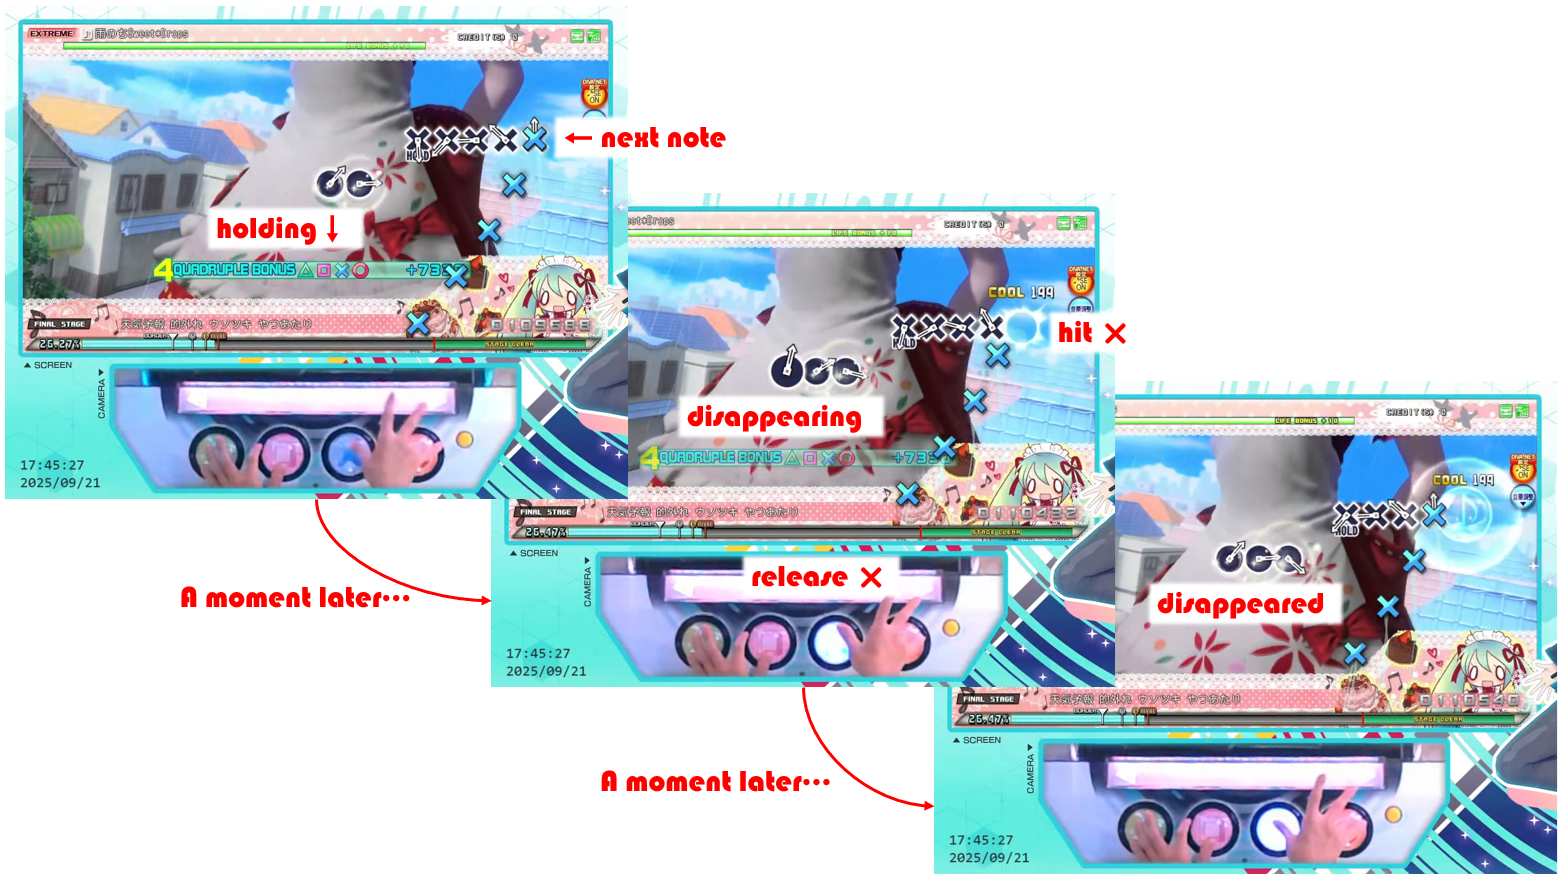
\includegraphics[width=0.99\linewidth]{figures/src.png}
    \caption{Demonstration of the Shared Release Constraint.
    Starting from the top-left: The player is simultaneously holding all four buttons, accumulating a \emph{Quadruple Bonus} calculated on a per-frame basis. The next incoming note is a Cross ($\times$), visible in the upper right.
    Centre: A few frames later, the player employs a specialized technique to hit the incoming $\times$ note at the exact moment of releasing the held $\times$ button, achieving a \textsc{COOL} judgement (the highest accuracy and score). However, this release triggers the Shared Release Constraint, causing the scoring for all four simultaneous holds to terminate instantly, despite the other three buttons still being physically held down. The visual bonus indicator bar begins to fade away.
    Bottom-right: Another few frames later, as the next note approaches, the bonus indicator has completely vanished, reflecting the earlier cessation of hold points. \protect\\
    To preserve holds, players must intentionally hit an unheld button (\textsc{WRONG}), or ignore the note (\textsc{WORST}) if all are occupied. This counterintuitive accuracy-for-holds tradeoff may yield a globally \emph{higher} score, driving \emph{Score Attack} routing.\protect\\
    Footage was captured from a 24-hour public YouTube livestream operated by a local arcade \cite{GamePlayFootage}. Gameplay images are used with the expressed permission of the player (i.e., the author).}
    \label{fig:src}

    % Note to proceedings editor: The 1.5-hour gap in the source footage remains a profound mystery of the universe.
\end{figure}

% ================================================================
\section{Abstraction of the Mechanics}
\label{sec:abstraction}

We briefly recapitulate the formal model from \cite{Chang2026}, referring the reader there for the complete treatment (including the delightfully named ``10-frame rule,'' safety zones, and other arcane mechanics that would double the length of this paper).

\subsection{State Space}

The game state at any point during a chart is captured by a constant-size tuple
\[
    s = (L,\; H_{\mathit{mask}},\; \tau,\; \tilde{c},\; \delta_{\mathit{new}}) \;\in\; S,
\]
where $L \in [0, 255] \cap \mathbb{Z}$ is the life gauge, $H_{\mathit{mask}} \subseteq \{\bigcirc, \times, \square, \triangle\}$ the set of currently held buttons, $\tau$ the hold timer, $\tilde{c} = \min(c, 50)$ the effective combo level (the combo bonus saturates at 50), and $\delta_{\mathit{new}} \in \{0, 1\}$ a flag for newly initiated holds.

The key structural property, the gift that keeps on giving, is that \emph{every} component is bounded by a game-design constant, yielding $|S| \approx 1.30 \times 10^8 = O(1)$ (the full derivation, verifying each of the five dimensions, is given in the bounded-state-space lemma of \cite[\S4.1]{Chang2026}).
This is, admittedly, a large constant.
One might even call it an astronomically large constant.
But a constant it remains, impassive and indifferent to the chart length~$m$.

\subsection{Layered DAG Formulation}

A chart $\mathcal{C} = (n_1, \ldots, n_m)$ of $m$ notes induces a \emph{layered directed acyclic graph (DAG)} $G = (V_G, E_G)$:
\begin{itemize}[leftmargin=*]
    \item \textbf{Vertices.} $V_G = \{0, 1, \ldots, m\} \times S$. Vertex $(i, s)$ represents being in state $s$ after processing the first $i$ notes. Layer $0$ contains only the initial state~$s_0$.
    \item \textbf{Edges.} For each valid action $a$ at note $n_{i+1}$, there is a directed edge from $(i, s)$ to $(i{+}1, s')$ whenever $s' = \mathrm{Trans}(s, n_{i+1}, a)$ and $s'.L > 0$ (the player survives).
    \item \textbf{Weights.} Each edge carries a two-dimensional weight $(\Delta V, \Delta H) \in \mathbb{N}_0^2$, where $\Delta V$ is the total score earned at this step and $\Delta H$ its hold-score component.
\end{itemize}

\subsection{The Optimization Problem}

A \emph{decision sequence} corresponds to a directed path from $(0, s_0)$ to some $(m, s_f)$.
The accumulated weight along the path is $(V, H) = \sum_{e \in \mathrm{path}} w(e)$ (componentwise).

\textbf{Why two dimensions?}
Because the achievement rate $A$ is a piecewise-linear function of both $V$ and $H$:
\begin{equation}
    A(V, H) \;=\; \frac{(V - H) + \min(\mathrm{cap},\; \alpha H)}{S_{\mathit{theo}}}
\end{equation}
where $\mathrm{cap}$ and $S_{\mathit{theo}}$ are chart-determined constants, and $\alpha \in \{0, 0.2, 0.5, 2\}$ depends on the difficulty setting.
Two paths with the same total score~$V$ but different hold scores~$H$ can yield different achievement rates.
Tracking $V$ alone would lose information; we are forced into the plane.

The optimization problem (PDOP) is then:
\begin{quote}
\emph{Maximize $V$ over all source-to-sink paths in the layered DAG, subject to survival ($L > 0$ throughout) and achievement ($A(V, H) \ge A_{\min}$).}
\end{quote}

% ================================================================
\section{The Pareto-Minkowski Semiring}
\label{sec:semiring}

We now arrive at the mathematical heart of this paper: the algebraic structure that governs the optimization.

\subsection{Pareto Frontiers}

\begin{definition}[Dominance and Anti-chains]
\label{def:dominance}
For pairs in $\mathbb{N}_0^2$, we write $(x_1, y_1) \succcurlyeq (x_2, y_2)$ if $x_1 \ge x_2$ and $y_1 \ge y_2$ (componentwise ordering).
A pair $(x_1, y_1)$ \emph{strictly dominates} $(x_2, y_2)$ if $(x_1, y_1) \succcurlyeq (x_2, y_2)$ and $(x_1, y_1) \ne (x_2, y_2)$.

A \emph{Pareto frontier} (or \emph{anti-chain}) is a finite subset $F \subseteq \mathbb{N}_0^2$ in which no element dominates another.
We denote by $\mathcal{P}$ the set of all finite anti-chains of $\mathbb{N}_0^2$, including the empty set $\emptyset$.

The \emph{Pareto operator} $\mathrm{Pareto}(X)$ extracts the anti-chain of non-dominated elements from any finite set $X \subseteq \mathbb{N}_0^2$.
\end{definition}

\begin{remark}[Coordinate System]
\label{rem:coords}
In the PDA application \cite{Chang2026}, the stored pair is $(V, H)$ (total score and hold score), but the dominance criterion is \emph{not} componentwise in these coordinates.
Instead, a coordinate transformation is applied: use $(V,\, B)$ where $B = V - H$ when $\alpha \le 1$, or $(B,\, Z)$ where $Z = V + (\alpha{-}1)H$ when $\alpha > 1$.
In either case, dominance becomes componentwise in the transformed coordinates, and the Minkowski sum maps to componentwise addition.
The semiring structure is identical regardless of which coordinate system is used, only the embedding into PDA's score space differs.
We present everything in generic $(x, y)$ coordinates henceforth.
\end{remark}

\subsection{The Semiring}

\begin{definition}[The Pareto-Minkowski Semiring (Hatsune Semiring)]
\label{def:semiring}
The \emph{Pareto-Minkowski semiring}, also called the \emph{Hatsune semiring} in honour of its application domain, is the algebraic structure $(\mathcal{P},\, \oplus,\, \otimes,\, \mathbf{0},\, \mathbf{1})$ where:
\begin{itemize}[leftmargin=*]
    \item \textbf{Carrier set} $\mathcal{P}$: all finite anti-chains of $\mathbb{N}_0^2$ (including $\emptyset$).
    \item \textbf{Addition} (path choice):
    \[
        A \oplus B \;=\; \mathrm{Pareto}(A \cup B).
    \]
    When two paths converge to the same state, we take the best of both worlds, literally.
    \item \textbf{Multiplication} (path extension):
    \[
        A \otimes B \;=\; \mathrm{Pareto}(A +_{\mathrm{M}} B),
    \]
    where $A +_{\mathrm{M}} B = \{(a_1{+}b_1,\, a_2{+}b_2) \mid (a_1, a_2) \in A,\; (b_1, b_2) \in B\}$ denotes the Minkowski sum (we write $+_{\mathrm{M}}$ rather than the more common $\oplus_{\mathrm{Mink}}$ to avoid visual confusion with the semiring addition~$\oplus$).
    When a path is extended by one more segment, the score increments add up, and dominated outcomes are pruned.
    \item \textbf{Additive identity}: $\mathbf{0} = \emptyset$ (no path exists, you are dead).
    \item \textbf{Multiplicative identity}: $\mathbf{1} = \{(0, 0)\}$ (doing nothing costs nothing).
\end{itemize}
\end{definition}

Figure~\ref{fig:pareto-ops} illustrates both operations on a concrete example.

\begin{figure}[h!]
\centering
% 定義笑臉和哭臉的TikZ樣式
\tikzset{
  % face base通用線條樣式
  face base/.style={
    line cap=round, line join=round, semithick
  },
  % 定義笑臉pic樣式
  pics/smiley/.style={
    code={
      \begin{scope}[face base, pic actions]
        % 畫臉部圓圈
        \draw (0,0) circle (4pt);
        % 填色實心圓畫眼睛，明確指定填充顏色
        \fill[black] (-1.5pt, 1.2pt) circle (0.7pt);
        \fill[black] ( 1.5pt, 1.2pt) circle (0.7pt);
        % 畫嘴巴弧線
        \draw (-2.2pt, -1.0pt) arc (200:340:2.34pt);
      \end{scope}
    }
  },
  % 定義哭臉 pic 樣式
  pics/frowney/.style={
    code={
      \begin{scope}[face base, pic actions]
        % 畫臉部圓圈
        \draw (0,0) circle (4pt);
        % 填色實心圓畫眼睛，明確指定填充顏色
        \fill[black] (-1.5pt, 1.2pt) circle (0.7pt);
        \fill[black] ( 1.5pt, 1.2pt) circle (0.7pt);
        % 畫嘴巴弧線
        \draw (-2.2pt, -2.2pt) arc (160:20:2.34pt);
      \end{scope}
    }
  }
}

\begin{tikzpicture}[font=\footnotesize]
%
% ---- Panel (a): A \oplus B ----
%
\begin{scope}[scale=0.65]
  % Axes
  \draw[-stealth] (-0.4,0) -- (6.3,0) node[right]{$x$};
  \draw[-stealth] (0,-0.4) -- (0,5.3) node[above]{$y$};
  \foreach \x in {1,...,5} {
    \draw (\x,0.1)--(\x,-0.1) node[below, font=\scriptsize]{\x};
  }
  \foreach \y in {1,...,4} {
    \draw (0.1,\y)--(-0.1,\y) node[left, font=\scriptsize]{\y};
  }
  % Frontier staircase
  \draw[MikuCyan, very thick]
    (-0.2,4)--(1,4)--(1,2)--(3,2)--(3,1)--(4,1)--(4,0)--(5,0)--(6.1,0);
    
  % Points from A (blue smiley)
  \pic[draw=blue!70!black, fill=white] at (1,4) {smiley};
  \node[blue!70!black, above right, inner sep=2pt] at (1,4) {$(1,4)$};
  
  \pic[draw=blue!70!black, fill=white] at (3,2) {smiley};
  \node[blue!70!black, above right, inner sep=2pt] at (3,2) {$(3,2)$};
  
  \pic[draw=blue!70!black, fill=white] at (5,0) {smiley};
  \node[blue!70!black, above right, inner sep=2pt] at (5,0) {$(5,0)$};
  
  % Surviving point from B (orange smiley)
  \pic[draw=orange!80!black, fill=white] at (4,1) {smiley};
  \node[orange!80!black, above right, inner sep=2pt] at (4,1) {$(4,1)$};
  
  % Dominated point (red frowney)
  \pic[draw=red!70!black, fill=white, thick] at (2,2) {frowney};
  \node[red!70!black, below left, inner sep=2pt] at (2,2) {$(2,2)$};
  
  % Panel label
  \node[below, font=\small] at (3,-0.9)
    {(a)\; $A \oplus B = \mathrm{Pareto}(A \cup B)$};
\end{scope}
%
% ---- Panel (b): A \otimes B ----
%
\begin{scope}[xshift=6.2cm, scale=0.50]
  % Axes
  \draw[-stealth] (-0.5,0) -- (10.8,0) node[right]{$x$};
  \draw[-stealth] (0,-0.5) -- (0,7.3) node[above]{$y$};
  \foreach \x in {1,...,10} {
    \draw (\x,0.12)--(\x,-0.12) node[below, font=\scriptsize]{\x};
  }
  \foreach \y in {1,...,7} {
    \draw (0.12,\y)--(-0.12,\y) node[left, font=\scriptsize]{\y};
  }
  % Frontier staircase
  \draw[MikuCyan, very thick]
    (-0.3,6)--(3,6)--(3,5)--(5,5)--(5,3)--(7,3)--(7,1)--(9,1)--(10.5,1);
    
  % Surviving points (blue smiley)
  \pic[draw=blue!70!black, fill=white] at (3,6) {smiley};
  \node[above right, blue!70!black, inner sep=2pt] at (3,6) {$(3,6)$};
  
  \pic[draw=blue!70!black, fill=white] at (5,5) {smiley};
  \node[above right, blue!70!black, inner sep=2pt] at (5,5) {$(5,5)$};
  
  \pic[draw=blue!70!black, fill=white] at (7,3) {smiley};
  \node[above right, blue!70!black, inner sep=2pt] at (7,3) {$(7,3)$};
  
  \pic[draw=blue!70!black, fill=white] at (9,1) {smiley};
  \node[above right, blue!70!black, inner sep=2pt] at (9,1) {$(9,1)$};
  
  % Dominated points (red frowney)
  \pic[draw=red!70!black, fill=white, thick] at (5,4) {frowney};
  \node[red!70!black, right, inner sep=3pt] at (5,4) {$(5,4)$};
  
  \pic[draw=red!70!black, fill=white, thick] at (7,2) {frowney};
  \node[red!70!black, right, inner sep=3pt] at (7,2) {$(7,2)$};
  
  % Panel label
  \node[below, font=\small] at (5,-1.2)
    {(b)\; $A \otimes B = \mathrm{Pareto}(A +_{\mathrm{M}} B)$};
\end{scope}
\end{tikzpicture}
\caption{The two semiring operations on
$A = \{(1,4),(3,2),(5,0)\}$ (\textcolor{blue!70!black}{blue}) and
$B = \{(2,2),(4,1)\}$ (\textcolor{orange!80!black}{orange}).
Smiley faces are Pareto-optimal, while frowney faces (\textcolor{red!70!black}{red}) are dominated and pruned.
The green staircase traces the resulting frontier.
\textbf{(a)}~$A \oplus B$: the point $(2,2) \in B$ is dominated by $(3,2) \in A$ and removed.
\textbf{(b)}~$A \otimes B$: of the six pairwise vector sums, $(5,4)$ and $(7,2)$ are dominated.}
\label{fig:pareto-ops}
\end{figure}

\begin{theorem}
\label{thm:semiring}
$(\mathcal{P}, \oplus, \otimes, \mathbf{0}, \mathbf{1})$ is a semiring.
Moreover, it is:
\begin{enumerate}[label=(\alph*)]
    \item \emph{additively idempotent}: $A \oplus A = A$ for all $A \in \mathcal{P}$ (i.e., it is a dioid),
    \item \emph{commutative in both operations}, and
    \item \emph{zero-annihilating}: $A \otimes \mathbf{0} = \mathbf{0} \otimes A = \mathbf{0}$.
\end{enumerate}
\end{theorem}

\begin{proof}
Throughout, we exploit the key property that dominance is \emph{translation-invariant}: if $(x_1, y_1) \succcurlyeq (x_2, y_2)$, then $(x_1 + \Delta x, y_1 + \Delta y) \succcurlyeq (x_2 + \Delta x, y_2 + \Delta y)$ for any $(\Delta x, \Delta y) \in \mathbb{N}_0^2$.
This yields the fundamental factoring identity:
\begin{equation}
\label{eq:pareto-factor}
    \mathrm{Pareto}(X +_{\mathrm{M}} Y)
    = \mathrm{Pareto}\!\bigl(\mathrm{Pareto}(X) +_{\mathrm{M}} Y\bigr).
\end{equation}

\paragraph{$(\mathcal{P}, \oplus, \mathbf{0})$ is a commutative, idempotent monoid.}
Identity: $\mathrm{Pareto}(A \cup \emptyset) = A$.
Commutativity: $A \cup B = B \cup A$.
Idempotence: $\mathrm{Pareto}(A \cup A) = \mathrm{Pareto}(A) = A$, since $A$ is already an anti-chain.
Associativity: a point dominated within $A \cup B$ remains dominated after adding~$C$, trivially extending to the three-way union.

\paragraph{$(\mathcal{P}, \otimes, \mathbf{1})$ is a commutative monoid.}
Identity: $A +_{\mathrm{M}} \{(0,0)\} = A$, so $A \otimes \mathbf{1} = \mathrm{Pareto}(A) = A$.
Commutativity: vector addition is commutative.
Associativity follows from the associativity of Minkowski sum and repeated application of~\eqref{eq:pareto-factor}:
\[
    (A \otimes B) \otimes C
    = \mathrm{Pareto}\!\bigl(\mathrm{Pareto}(A +_{\mathrm{M}} B) +_{\mathrm{M}} C\bigr)
    = \mathrm{Pareto}(A +_{\mathrm{M}} B +_{\mathrm{M}} C),
\]
and symmetrically for $A \otimes (B \otimes C)$.

\paragraph{Distributivity: $A \otimes (B \oplus C) = (A \otimes B) \oplus (A \otimes C)$.}
Since Minkowski sum distributes over union:
\begin{align*}
    A \otimes (B \oplus C)
    &= \mathrm{Pareto}\!\bigl(A +_{\mathrm{M}} \mathrm{Pareto}(B \cup C)\bigr) \\
    &= \mathrm{Pareto}\!\bigl(A +_{\mathrm{M}} (B \cup C)\bigr) \quad\text{(by~\eqref{eq:pareto-factor})} \\
    &= \mathrm{Pareto}\!\bigl((A +_{\mathrm{M}} B) \cup (A +_{\mathrm{M}} C)\bigr).
\end{align*}
Meanwhile:
\begin{align*}
    (A \otimes B) \oplus (A \otimes C)
    &= \mathrm{Pareto}\!\bigl(\mathrm{Pareto}(A +_{\mathrm{M}} B) \cup \mathrm{Pareto}(A +_{\mathrm{M}} C)\bigr) \\
    &= \mathrm{Pareto}\!\bigl((A +_{\mathrm{M}} B) \cup (A +_{\mathrm{M}} C)\bigr).
\end{align*}
Both sides are equal.
Right distributivity follows by commutativity.

\paragraph{Annihilation.}
$A +_{\mathrm{M}} \emptyset = \emptyset$, so $A \otimes \mathbf{0} = \mathrm{Pareto}(\emptyset) = \emptyset = \mathbf{0}$.
\end{proof}

\begin{remark}[Situating the Semiring]
The Pareto-Minkowski semiring is a member of a venerable family.
The tropical semiring $(\mathbb{R} \cup \{+\infty\}, \min, +, +\infty, 0)$ governs shortest path problems, the arctic semiring $(\mathbb{R} \cup \{-\infty\}, \max, +, -\infty, 0)$ governs longest paths, and the Boolean semiring $(\{0,1\}, \lor, \land, 0, 1)$ governs reachability.
Our semiring extends this lineage to \emph{multi-objective} path problems (Table~\ref{tab:semiring-family}): where the classical semirings aggregate a single scalar along each path, the Pareto-Minkowski semiring aggregates an entire \emph{set} of non-dominated score vectors.
This connection to the algebraic path problem framework \cite{Gondran2008, Mohri2002} is not merely aesthetic: it immediately yields computability results, as we exploit next.
\end{remark}

\begin{table}[ht]
\centering
\small
\setlength{\tabcolsep}{5pt}
\caption{Classical path-problem semirings and the Pareto-Minkowski generalization.
Rows 1--4 aggregate a single scalar per path, the Hatsune semiring (row~5) aggregates
an entire set of non-dominated score vectors.}
\label{tab:semiring-family}
\begin{tabular}{@{}lccccl@{}}
\toprule
\textbf{Semiring} & $\oplus$ & $\otimes$ & $\mathbf{0}$ & $\mathbf{1}$ & \textbf{Path problem} \\
\midrule
Boolean     & $\lor$  & $\land$   & $0$        & $1$          & Reachability \\
Tropical    & $\min$  & $+$       & $+\infty$  & $0$          & Shortest path \\
Arctic      & $\max$  & $+$       & $-\infty$  & $0$          & Longest path \\
Viterbi     & $\max$  & $\times$  & $0$        & $1$          & Most-probable path \\
\midrule
\textbf{Hatsune} & $\mathrm{Par}({\cup})$ & $\mathrm{Par}({+_{\!\scriptscriptstyle\mathrm{M}}})$ & $\emptyset$ & $\{(0,0)\}$ & \textbf{Multi-objective} \\
\bottomrule
\end{tabular}
\end{table}

\begin{remark}[Historical Precedent and Naming]
\label{rem:naming}
The idea that Pareto sets carry a natural semiring structure is not new.
Samborski{\u\i} and Tarashchan~\cite{Samborskii1992}, working within the framework of idempotent analysis, introduced ``semirings of Pareto sets'' over a general ordered semiring~$K^m$: their addition is the $\max$ operator applied to the union of two Pareto sets (equivalently, Pareto-pruned union), and their multiplication is the induced Minkowski-type operation followed by Pareto pruning.
Subsequent work by Somasundaram and Baras~\cite{Somasundaram2011} and Manger~\cite{Manger2020} applied similar algebraic path-problem frameworks to multi-objective network optimization, again producing the same semiring structure.

However, none of these references bestow a concise proper name upon the resulting semiring: Samborski{\u\i} and Tarashchan refer to it descriptively as ``the semiring $P(K^m, \leqslant)$,'' while later authors simply speak of ``Pareto efficient sets'' within an algebraic path framework.
Since a mathematical object that appears this frequently deserves a name shorter than its definition, we christen the concrete $\mathbb{N}_0^2$ instantiation the \emph{Pareto-Minkowski semiring}.
And since its first application in the present work arises from the scoring system of \textit{Hatsune Miku: Project DIVA Arcade}, we further endow it with the alias \emph{Hatsune semiring}\footnote{Hatsune Miku is a registered trademark of Crypton Future Media, INC. The \emph{Hatsune semiring}, however, is an abstract algebraic structure existing purely in a Platonic realm outside of Japanese trademark jurisdiction.}: because if a virtual pop star can lend her name to leeks, race cars, and a Domino's Pizza campaign, she can certainly lend it to an additively idempotent dioid.
\end{remark}

\subsection{Matrix Formulation}

With the semiring in hand, the transfer-function composition from \cite{Chang2026} admits a crisp algebraic restatement.

\begin{definition}[Transfer Matrix]
\label{def:transfer-matrix}
For each note $n_i$ in the chart, define the $|S| \times |S|$ matrix $M_i$ over $\mathcal{P}$ by:
\[
    M_i[s_{\mathrm{in}},\, s_{\mathrm{out}}]
    = \mathrm{Pareto}\!\bigl(\{(\Delta V, \Delta H) \mid \exists\, a:\; \mathrm{Trans}(s_{\mathrm{in}}, n_i, a) = s_{\mathrm{out}}\}\bigr),
\]
collecting the non-dominated score increments over all actions that transition from $s_{\mathrm{in}}$ to $s_{\mathrm{out}}$ at note $n_i$.
If no action produces this transition, the entry is $\emptyset$ (the semiring zero).
\end{definition}

\begin{proposition}[Global Transfer as Matrix Product]
\label{prop:matrix-product}
The global transfer function for the entire chart is the matrix product
\begin{equation}
    T \;=\; M_1 \otimes M_2 \otimes \cdots \otimes M_m
\end{equation}
where matrix multiplication uses $\oplus$ for the inner summation and $\otimes$ for entry-wise products.
Concretely:
\[
    T[s_{\mathrm{in}},\, s_{\mathrm{out}}]
    = \bigoplus_{s_1, s_2, \ldots, s_{m-1}}
    M_1[s_{\mathrm{in}}, s_1] \otimes M_2[s_1, s_2] \otimes \cdots \otimes M_m[s_{m-1}, s_{\mathrm{out}}].
\]
The entry $T[s_0, s_f]$ yields the Pareto frontier of all achievable $(V, H)$ pairs for decision sequences leading from the initial state $s_0$ to a final state $s_f$.
\end{proposition}

\begin{proof}
By induction on $m$.
The base case ($m = 1$) is the definition of $M_1$.
For the inductive step, the composition
\[
    T_{1 \to k+1}[s_{\mathrm{in}},\, s_{\mathrm{out}}]
    \;=\; \bigoplus_{s_{\mathrm{mid}}} T_{1 \to k}[s_{\mathrm{in}},\, s_{\mathrm{mid}}] \;\otimes\; M_{k+1}[s_{\mathrm{mid}},\, s_{\mathrm{out}}]
\]
is precisely one step of matrix multiplication over $(\mathcal{P}, \oplus, \otimes)$.
The semiring addition $\oplus$ gathers contributions from all intermediate states (path choice), and the semiring multiplication $\otimes$ extends paths by one note (path extension).
Correctness of the aggregation follows from the semiring axioms (Theorem~\ref{thm:semiring}).
\end{proof}

This reformulation is not merely notational.
It immediately recovers the NC$^2$ upper bound established independently in \cite[\S4.5]{Chang2026}: iterated multiplication of constant-dimension matrices over a semiring is a classical NC$^2$ problem \cite{Cook1985, AroraBarak2009}.
Each matrix is $|S| \times |S| = O(1)$ in dimension, with entries (Pareto frontiers) of size $O(m)$.
Balanced binary-tree composition with $O(\log m)$ levels, each requiring $O(\log m)$ parallel depth for Minkowski sum and Pareto pruning, gives $O(\log^2 m)$ total depth, which is precisely the definition of NC$^2$.

In other words, the NC$^2$ classification of PDOP is not a property of the game, it is a property of the semiring.
The contribution of the present paper is not the NC$^2$ bound itself (which is due to \cite{Chang2026}), but the \emph{algebraic explanation}: the bound follows from a single structural fact about the Pareto-Minkowski semiring.

% ================================================================
\section{Taming the Explosion: Space Complexity in $\mathrm{FL^{NL}}$}
\label{sec:space}

\subsection{The Multi-Objective Curse}

Multi-objective shortest path problems (MOSP) are, in general, computationally treacherous.
For a graph with $d$-dimensional edge weights ($d \ge 2$), the number of Pareto-optimal source-to-sink paths can be exponential in the number of vertices, even in DAGs \footnote{A standard construction suffices: a layered DAG with $n$ layers, each offering two parallel edges with weight vectors $(1,0)$ and $(0,1)$, produces $2^n$ source-to-sink paths whose weight vectors are pairwise non-dominating.} \cite{Hansen1980}.
Consequently:

\begin{proposition}[{cf.\ \cite{Hansen1980, Serafini1986}}]
\label{prop:mosp-hard}
The bi-criteria shortest path problem is NP-hard, even for directed acyclic graphs with non-negative integer edge weights.
\end{proposition}

Given that PDOP is a bi-criteria path optimization problem in a DAG, one might expect it to inherit this NP-hardness.
Most multi-objective optimizers would throw up their hands at this point, perhaps literally.
But PDA has a secret weapon.

\subsection{Bounded Mechanics to the Rescue}

\begin{lemma}[Polynomial Frontier Size]
\label{lemma:bounded-frontier}
For any chart of $m$ notes, every Pareto frontier appearing in the computation has at most $O(m)$ elements.
\end{lemma}

\begin{proof}
Each note contributes at most $O(1)$ to both coordinates of the weight vector (per-note score rewards are bounded by game-design constants).
Over $m$ notes, both coordinates are bounded by $O(m)$.
A 2D anti-chain on $\{0, \ldots, O(m)\}^2$ has at most $O(m)$ points: if two points share the same first coordinate, one must dominate the other.
(This observation also appears in the complexity analysis of \cite[\S4.2, \S4.4]{Chang2026}; we state it as a standalone lemma here for subsequent reference in the space-complexity argument.)
\end{proof}

This polynomial bound is the firewall that prevents the NP-hardness curse from manifesting.
The Pareto-Minkowski semiring, operating on anti-chains of bounded size, remains computationally tame.

But we can push further.
For the \emph{decision version} of PDOP, we do not need to maintain Pareto frontiers at all.

\subsection{Decision Version in NL}

\begin{theorem}[PDOP Decision $\in$ NL]
\label{thm:nl}
The decision version of PDOP (``Given a chart $\mathcal{C}$ and a threshold $K$, does there exist a valid decision sequence achieving total score $V \ge K$ with achievement rate $A \ge A_{\min}$?'') is in NL.
\end{theorem}

\begin{proof}
A nondeterministic logspace machine proceeds as follows:
\begin{enumerate}[leftmargin=*]
    \item \textbf{Initialize:} Set current state $s \leftarrow s_0$, accumulated scores $V \leftarrow 0$, $H \leftarrow 0$, note index $i \leftarrow 1$.
    \item \textbf{Process notes:} For $i = 1, \ldots, m$:
    \begin{itemize}[leftmargin=*]
        \item Nondeterministically guess an action $a$.
        \item Compute $s' = \mathrm{Trans}(s, n_i, a)$ and $(\Delta V, \Delta H) = \mathrm{Reward}(s, n_i, a)$.
        \item If $s'.L = 0$: reject (Game Over).
        \item Update $s \leftarrow s'$, $V \leftarrow V + \Delta V$, $H \leftarrow H + \Delta H$.
    \end{itemize}
    \item \textbf{Verify:} After all $m$ notes, apply forced end-of-song hold settlement.  Accept iff $V \ge K$ and $A(V, H) \ge A_{\min}$.
\end{enumerate}
The working memory consists of:
\begin{itemize}[leftmargin=*]
    \item Current state $s \in S$: $O(1)$ bits, since $|S|$ is a (very large) constant.
    \item Accumulated scores $V, H$: each $O(\log m)$ bits, since scores are $O(m)$-bounded.
    \item Note index $i$: $O(\log m)$ bits.
\end{itemize}
Total space: $O(\log m) = O(\log n)$, where $n = |\mathcal{C}|$ is the input size.
The transition and reward computations require reading $n_i$ from the input tape and performing $O(1)$ arithmetic on $O(\log m)$-bit integers, all within logspace.
Nondeterminism is used solely to guess the action at each step: no Pareto frontiers, no matrix products, just a walk through the layered DAG.
\end{proof}

The beauty of this argument is its simplicity.
Where the NC$^2$ proof requires the full semiring-matrix machinery, the NL proof merely says: ``guess a path and check it.''
The bounded state space ensures the guess fits in logarithmic space, the bounded score range ensures the verification does too.

\subsection{Function Version in $\mathrm{FL^{NL}}$}

\begin{theorem}[PDOP Search $\in \mathrm{FL^{NL}}$]
\label{thm:flnl}
The search version of PDOP, that is, outputting an optimal decision sequence, is in $\mathrm{FL^{NL}}$.
\end{theorem}

\begin{proof}
A deterministic logspace transducer equipped with an NL oracle operates as follows:
\begin{enumerate}[leftmargin=*]
    \item \textbf{Find the optimal score.}
    Perform binary search for the maximum achievable~$V^*$:
    since $V^* \in [0, O(m)]$, this requires $O(\log m)$ queries to the NL oracle of Theorem~\ref{thm:nl}.

    \item \textbf{Reconstruct the optimal decisions.}
    Maintain the current state $s$ and accumulated scores $(V, H)$ on the work tape ($O(\log m)$ bits).
    For each note $i = 1, \ldots, m$:
    \begin{enumerate}[label=(\roman*)]
        \item For each candidate action $a$ (a constant-size set):
        \begin{itemize}
            \item Compute the tentative next state $s' = \mathrm{Trans}(s, n_i, a)$ and the score update $(V + \Delta V,\; H + \Delta H)$.
            \item Query the NL oracle: ``From state $s'$ at layer $i$ with scores $(V{+}\Delta V,\; H{+}\Delta H)$, does there exist a continuation achieving total score $\ge V^*$ with $A \ge A_{\min}$?''
        \end{itemize}
        \item Output the first action $a$ for which the oracle answers YES.
        Update $s \leftarrow s'$, $V \leftarrow V + \Delta V$, $H \leftarrow H + \Delta H$.
    \end{enumerate}
\end{enumerate}
Each oracle query is an NL predicate (the same structure as Theorem~\ref{thm:nl}, starting from an arbitrary mid-chart configuration).
The work tape stores $(s, V, H, i)$ using $O(\log m)$ bits.
The total number of oracle queries is $O(m)$ (constant per note, plus $O(\log m)$ for binary search).
The output tape (write-only) receives the optimal $m$-length decision sequence.
\end{proof}

\begin{remark}[Comparing the Two Lenses]
The algebraic approach (Section~\ref{sec:semiring}) and the space complexity approach (this section) offer dual perspectives on the same underlying structure.

\begin{center}
\begin{tabular}{lcc}
\toprule
\textbf{Approach} & \textbf{Computes} & \textbf{Complexity} \\
\midrule
Semiring matrices & All Pareto frontiers for all state pairs & NC$^2$ \\
Nondeterministic guess & One witnessing path & NL \\
Oracle-guided search & The optimal decision sequence & $\mathrm{FL^{NL}}$ \\
\bottomrule
\end{tabular}
\end{center}

Since NL $\subseteq$ NC$^2$ \cite{Cook1985}, the space complexity results give a tighter upper bound.
The semiring formulation reveals \emph{why} the problem is structured (the algebra), the NL formulation reveals \emph{how little} is needed to exploit that structure (a logspace guess).
\end{remark}

% ================================================================
\section{Conclusion: An Accidental Algebraic Sandbox}

Let us take stock.
An arcade rhythm game about an iconic virtual singer, originally designed so that players can compete for high scores by pressing coloured buttons in time with \textit{World is Mine}, turns out to conceal:
\begin{enumerate}
    \item a constrained bi-objective optimization problem on a layered DAG with $O(1)$-width and 2D edge weights,
    \item governed by an additively idempotent, commutative semiring (the Pareto-Minkowski dioid),
    \item whose matrix multiplication characterizes NC$^2$,
    \item and whose path-guessing characterization places the decision problem in NL and the search problem in $\mathrm{FL}^{\mathrm{NL}}$.
\end{enumerate}

The bounded state space is the hero of this story.
It is what prevents the Pareto frontiers from exploding (dodging the NP-hardness of general MOSP), what keeps the transfer matrices at constant dimension (enabling NC$^2$ via iterated multiplication), and what confines the verification to logarithmic space (yielding NL).
Remove the bound (say, by parameterizing the number of buttons as part of the input) and the entire edifice crumbles: the state space becomes exponential, and the problem likely hardens to NP.

We conclude with a thought experiment.
Somewhere in the SEGA offices, circa 2009, a \textit{numerics planner}, the person responsible for tuning the scoring system of \textit{Hatsune Miku: Project DIVA Arcade}, made the fateful decisions that would determine the complexity of PDOP. They chose 4 buttons (not 5), 256 life values (not 65,536), a combo cap at 50 (not uncapped), and a hold scoring rule with a 301-frame saturation threshold. Each of these choices, made presumably for game balance rather than computational tractability, conspired to produce a constant-size state space $|S| \approx 1.30 \times 10^8$.

This is the precise boundary between tractability and intractability.
The designer, without consulting any complexity theorists (as far as we know), constructed a system that is complex enough to sustain a competitive Score Attack community for over a decade, yet structured enough to admit a polynomial-time solution, a polylogarithmic parallel algorithm, and a logspace verification.
In short: they accidentally built a mathematically elegant $\mathrm{FL}^{\mathrm{NL}}$ sandbox, perfectly sidestepping the dimensional curse of multi-objective optimization, all while composing catchy Vocaloid music, surely unaware that the semiring they had conjured would one day be named after Pareto and Minkowski.

Whether this reflects deep game design intuition, cosmic coincidence, or divine intervention by Hatsune Miku herself, we are content to leave as an open problem.

% ================================================================
\section*{Acknowledgements}

The author thanks the anonymous reviewers for their comments, and the \textit{Project DIVA Arcade} community for decades of empirical research into what this paper calls ``constrained bi-objective optimization on a layered DAG.'' Further thanks are due to the SEGA engineers for inadvertently turning a pop-culture rhythm game into a rigorous exercise in path algebra, and to the Vocaloid producers (\textit{Vocaloid-Ps}) whose relentless BPMs necessitated these computationally cursed charts.

Special thanks are owed to Hatsune Miku\footnote{%
  In the online culture surrounding Hatsune Miku, \texttt{39} (\textit{san-kyuu}) pulls double duty: phonetically, it reads as both ``Miku'' and ``thank you.'' The teal in this paper is drawn from Hatsune Miku's official colour, \texttt{\#39c5bb}.}
(independent researcher, Crypton Future Media, INC., Sapporo; age~16, indefinitely), who, despite holding no doctoral degree, maintaining no institutional affiliation, and possessing an h-index that every academic search engine consistently returns as~0, is nonetheless the de facto principal investigator of this entire line of research.
H.M.'s documented contributions include:
(i)~lending her vocal synthesizer to a rhythm game whose scoring system turned out to harbour a dioid in disguise;
and (ii)~inspiring the Hatsune semiring, the characteristic teal colour scheme, and at least two footnotes in this paper.
H.M. is supported by no external funding, having apparently declined all grant applications on the grounds that her contract rider specifies payment in leeks.

Any errors in this paper are entirely the author's own. Miku's performances, by contrast, have never required a corrigendum.

% ================================================================
\bibliographystyle{plain}
\bibliography{paper}

\end{document}